\documentclass{article}
\usepackage{tikz}
\usetikzlibrary{arrows.meta,positioning,calc,shapes.geometric}
\pagestyle{empty}
\begin{document}
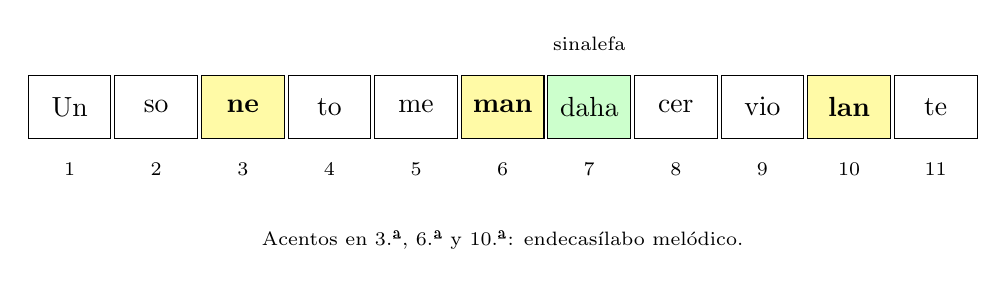
\begin{tikzpicture}

\def\s#1#2#3{\node[draw, minimum width=1.05cm, minimum height=0.8cm, fill=#3] at (#1,0) {#2};}
\s{0}{Un}{white}\s{1.1}{so}{white}\s{2.2}{\textbf{ne}}{yellow!35}\s{3.3}{to}{white}\s{4.4}{me}{white}\s{5.5}{\textbf{man}}{yellow!35}\s{6.6}{daha}{green!20}\s{7.7}{cer}{white}\s{8.8}{vio}{white}\s{9.9}{\textbf{lan}}{yellow!35}\s{11.0}{te}{white}
\foreach \i/\n in {0/1,1.1/2,2.2/3,3.3/4,4.4/5,5.5/6,6.6/7,7.7/8,8.8/9,9.9/10,11.0/11} {\node[font=\scriptsize] at (\i,-0.8) {\n};}
\node[font=\scriptsize] at (6.6,0.8) {sinalefa};
\node[font=\scriptsize, align=center] at (5.5,-1.7) {Acentos en 3.ª, 6.ª y 10.ª: endecasílabo melódico.};

\end{tikzpicture}
\end{document}
